\chapter{Simulation Environment}
\label{chap:Simulation}
In order to implement and research various FDIR systems on satellites, a simulation of satellite dynamics and kinematics is developed. The focus of this thesis is directed towards small satellites and, more specifically, CubeSats. During the development of the satellite simulation,\cite{auret2012design, JansevanVuuren2015, Jordaan2016, jeger2017determination} were frequently referenced. The simulation was developed in Python to simulate the dynamics and kinematics during a satellite orbit.

\section{Satellite Orbit Fundamentals}

 The main operational goal of the ADCS on this specific satellite mission is to control the payload so that it points towards the centre of the Earth during an eclipse and points the solar panels towards the sun during the sunlit phase. To ensure this is accurately simulated, the different coordinate frames dominating a satellite orbit, the attitude of the satellite, as well as the satellite dynamics and kinematics is discussed in this section.

\subsection{Coordinate Frames}
\label{section:CoordinateFrames}
The coordinate frames in aerospace is a fundamental part of the ADCS. In order to determine the orientation and position of an object, it should be relative to a fixed frame. Consequently, the Earth inertial coordinate (EIC) frame, $\mathcal{E}\{\bar{\mathbf{x}}_{\mathcal{E}},~\bar{\mathbf{y}}_{\mathcal{E}},~\bar{\mathbf{z}}_{\mathcal{E}}\}$, is the fixed frame from which every other frame is relative to.

A coordinate frame, $\mathcal{A}$, consists of three orthogonal vectors which is commonly referred to as $\bar{\mathbf{x}}_\mathcal{A}$, $\bar{\mathbf{y}}_\mathcal{A}$, and $\bar{\mathbf{z}}_\mathcal{A}$. The axes of the coordinate frame is appropriately named as the X-axis, Y-axis and Z-axis. A vector ($\mathbf{r}_\mathcal{A}$) within the coordinate frame can thus be expressed as 
\begin{equation}
\mathbf{r}_\mathcal{A} = a\bar{\mathbf{x}}_\mathcal{A} + b\bar{\mathbf{y}}_\mathcal{A} + c\bar{\mathbf{z}}_\mathcal{A},
\end{equation}
where the magnitude of $\mathbf{r}$, denoted as $\norm{\mathbf{r}}$, is equal to 
\begin{equation}
\norm{\mathbf{r}} = \sqrt{a^2 + b^2 + c^2}.
\end{equation}

The Earth-centered coordinate frames are dived into two, namely the EIC and Earth fixed coordinate (EFC) frame, $\mathcal{F}\{\bar{\mathbf{x}}_{\mathcal{F}},~\bar{\mathbf{y}}_{\mathcal{F}},~\bar{\mathbf{z}}_{\mathcal{F}}\}$. EFC is fixed to the Earth and rotates with it, while EIC is inertial fixed.

% Insert a figure of the Earth coordinate frames here

The EIC is defined as the Z-axis pointing towards the north pole, the X-axis pointing towards the Vernal Equinox, $\Upsilon$, and the Y-axis completing the orthogonal set. The EFC is a copy of the EIC, with the Z-axis being identical. The EFC, however, rotates with the Earth. The EFC in relation to the EIC can be expressed by a single angle of rotation, which is the Greenwich Hour Angle (GHA), $\alpha_G$. With the elapsed time, $t$, since $t_0$, the angular rate of the Earth, $\omega_E$, and the GHA, $\alpha_{G_0}$, at $t = t_0$ known, $\alpha_G$ can be calculated as 
\begin{equation}
\alpha_G = \omega_Et + \alpha_{G_0}.
\end{equation}
To transform a vector from one coordinate frame to another, a transformation matrix, $\boldsymbol{A}$, is required. For example vector $\mathbf{r}_{\mathcal{F}}$ can be transformed to $\mathbf{r}_{\mathcal{E}}$ with 
\begin{equation}
\mathbf{r}_{\mathcal{E}} = \boldsymbol{A}^{\mathcal{E}}_{\mathcal{F}}\mathbf{r}_{\mathcal{F}}
\end{equation}
with $\boldsymbol{A}^{\mathcal{E}}_{\mathcal{F}}$ being the EFC-to-EIC transformation matrix. Due to the definition of both coordinate frames, $\boldsymbol{A}^{\mathcal{E}}_{\mathcal{F}}$ can be defined as

\begin{equation}
\boldsymbol{A}^{\mathcal{E}}_{\mathcal{F}} = 
\begin{bmatrix}
	\text{cos}(\alpha_G) & -\text{sin}(\alpha_G) & 0\\
	\text{sin}(\alpha_G) & \text{cos}(\alpha_G) & 0 \\
	0 & 0 & 1
\end{bmatrix}.
\end{equation}
To determine the satellite position, satellite-centred coordinate frames must be used. Three satellite-centred coordinate frames are used, namely the inertial-reference coordinate frame (IRC), $\mathcal{I}\{\bar{\mathbf{x}}_{\mathcal{I}},~\bar{\mathbf{y}}_{\mathcal{I}},~\bar{\mathbf{z}}_{\mathcal{I}}\}$,  which remains inertial fixed, the orbit-referenced coordinate (ORC) frame, $\mathcal{O}\{\bar{\mathbf{x}}_{\mathcal{O}},~\bar{\mathbf{y}}_{\mathcal{O}},~\bar{\mathbf{z}}_{\mathcal{O}}\}$ and the satellite body coordinate (SBC) frame, $\mathcal{B}\{\bar{\mathbf{x}}_{\mathcal{B}},~\bar{\mathbf{y}}_{\mathcal{B}},~\bar{\mathbf{z}}_{\mathcal{B}}\}$. 
% The IRC frame is only acknowledged, since it is the frame that is fixed (as it does not rotate around the centre of the satellite), however it changes position with the orbit of the satellite. This frame is not used to determine the position of the satellite and will not be referenced for the remainder of this document.

The ORC frame changes location as the satellite move. The Z-axis is, however, always pointing towards the centre of the Earth, with the Y-axis being the orbit anti-normal and the X-axis completing the orthogonal set. To transform a vector from the EIC frame to the ORC frame the unit position vector, $\mathbf{r}_{sat}$ and the unit velocity vector, $\mathbf{v}_{sat}$ in EIC is required \cite{Chen_ground-target}. The EIC to ORC transformation matrix, $\boldsymbol{A}^{\mathcal{O}}_{\mathcal{E}}$, is calculate as
\begin{equation}
\label{Eq: ORC to EIC}
\begin{aligned}
	\boldsymbol{A}^{\mathcal{O}}_{\mathcal{E}} &= 
	\begin{bmatrix}
		\mathbf{u} & \mathbf{v} & \mathbf{w}\\
	\end{bmatrix}^T \\
\text{where} \quad
\mathbf{w} &= -\frac{\mathbf{r}_{sat}}{\norm{\mathbf{r}_{sat}}} \\
\mathbf{v} &= -\frac{\mathbf{r}_{sat} \times \mathbf{v}_{sat}}{\norm{\mathbf{r}_{sat} \times \mathbf{v}_{sat}}} \\
\mathbf{u} &= \mathbf{v} \times \mathbf{w}. \\
\end{aligned}
\end{equation}

The SBC frame is the frame fixed to the satellite and it is the relative rotation of the satellite in relation to the ORC. Thus for the mission of this satellite it is required that the SBC and ORC frames coincide during an eclipse. For the transformation of a vector from the ORC to SBC frame, the direct cosine matrix (DCM), also referred to as $\boldsymbol{A}$ or $\boldsymbol{A}^{\mathcal{B}}_{\mathcal{O}}$, is used. For the remainder of the document the DCM will be referred to as $\boldsymbol{A}^{\mathcal{B}}_{\mathcal{O}}$ to avoid any confusion. The calculation of this transformation matrix is discussed in $\S$\ref{subsection_quaternions} and implemented with Eq~\ref{eq:DCM_quaternion}.

% Insert a figure of the satellite coordinate frames here

\subsection{Attitude}
\label{subsection_quaternions}
To determine the attitude of an object, a mathematical model must be used to determine the rotation of an object in three dimensions. For this the visual and intuitive example of the Euler angles exist. Euler angles are the rotation of an object around three orthogonal axes which change orientation with the rotation of the object. The three axes of SBC, denoted by $\bar{\mathbf{x}}_{\mathcal{B}}$, $\bar{\mathbf{y}}_{\mathcal{B}}$ and $\bar{\mathbf{z}}_{\mathcal{B}}$ rotate with the object as depicted in Figure~\ref{fig:Pitch}.
\begin{figure}[!htb]
	\centering
	\def\svgwidth{10cm}
	\import{Figures/}{Pitch.pdf_tex}
	\caption{Euler angles}
	\label{fig:Pitch}
\end{figure}

$\boldsymbol{A}^{\mathcal{B}}_{\mathcal{O}}$ can be used to calculate the attitude transformation from given Euler angle rotations. This is done by multiplying the transformation matrices representing each individual Euler angle rotation. $\boldsymbol{A}^{\mathcal{B}}_{\mathcal{O}}$ can therefore be calculated as 
\begin{equation}
	\begin{aligned}
		\boldsymbol{A}^{\mathcal{B}}_{\mathcal{O}} &= \boldsymbol{A}_{\psi} \boldsymbol{A}_{\phi} \boldsymbol{A}_{\theta} \\
			&= \begin{bmatrix}
			\text{cos}(\psi) & \text{sin}(\psi) & 0 \\
			-\text{sin}(\psi) & \text{cos}(\psi) & 0 \\
			0 & 0 & 1
			\end{bmatrix} \begin{bmatrix}
			1 & 0 & 0 \\
			0 & \text{cos}(\phi) & \text{sin}(\phi) \\
			0 & -\text{sin}(\phi) & \text{cos}(\phi)
			\end{bmatrix} \begin{bmatrix}
			\text{cos}(\theta) &  0 & -\text{sin}(\theta) \\
			0 & 1 & 0 \\
			\text{sin}(\theta) & 0 & \text{cos}(\theta)
			\end{bmatrix}. \\
	\end{aligned}
\end{equation}
Euler angles, however, does not always prove a suitable method for determining the attitude of a satellite. This is due to singularities that can occur, such as the gimbal-lock effect, where two rotational axes coincide to form a single rotational axis. Consequently, not all $3$D rotations can be described with Euler angles, because with gimbal-lock only two effective rotations can occur instead of three \cite{diebel2006representing}. The method of describing $3$D rotation with quaternions is therefore more convenient and more often used. 

A quaternion, $\mathbf{q}$, has four components that are dependent on one another and constrained by 
\begin{equation} 
\label{Eq-quaternion dependency}
q_1^2 + q_2^2 + q_3^2 + q_4^2 = 1.
\end{equation}
The attitude quaternion is also related to the Euler angles in that if the Euler rotational axis from ORC to SBC is defined as a unit vector $\mathbf{e} = \begin{bmatrix} e_1  & e_2 & e_3 \end{bmatrix}^T$ and the angle of the Euler rotation is $\Phi$ then $\mathbf{q}$ can be expressed as
\begin{equation}
\mathbf{q} = \begin{bmatrix} e_1 \text{sin}(\frac{\Phi}{2}) \\ e_2 \text{sin}(\frac{\Phi}{2}) \\ e_3 \text{sin}(\frac{\Phi}{2}) \\ \text{cos}(\frac{\Phi}{2}) \end{bmatrix}
\end{equation}
Although it is difficult to visualize a quaternion, the most simplistic method of conceptualising it is shown in Figure~\ref{fig:quaternion}. A quaternion can be simplified to a unit vector protruding from the centre point of an object as well as the angle of rotation of that object around the unit vector. As seen in Figure~\ref{fig:Pitch} the angle $\theta$ is the angle of rotation around the $\bar{\mathbf{z}}_\mathcal{B}''$-axis. For quaternions the angle of rotation is the same principle, however, the axis around which the object is rotating, is the unit vector, $q_{1-3}$. Therefore, $q_4$ provides the angle of rotation while $q_{1-3}$ represents the unit vector, however, with the condition of Eq~\ref{Eq-quaternion dependency}.

\begin{figure}[!htb]
	\centering
	\def\svgwidth{10cm}
	\import{Figures/}{quaternion.pdf_tex}
	\caption{Graphical quaternion representation}
	\label{fig:quaternion}
\end{figure}

$\boldsymbol{A}^{\mathcal{B}}_{\mathcal{O}}$ can also be transformed as a function of $\mathbf{q}$ \cite{wertz2012spacecraft} through

\begin{equation}
\label{eq:DCM_quaternion}
	\boldsymbol{A}^{\mathcal{B}}_{\mathcal{O}}
		= \begin{bmatrix}
		q_1^2 - q_2^2 - q_3^2 + q_4^2 & 2(q_1q_2 + q_3q_4) & 2(q_1q_3 - q_2q_4) \\
		2(q_1q_2 - q_3q_4) & -q_1^2 + q_2^2 - q_3^2 + q_4^2 & 2(q_2q_3 + q_1q_4) \\
		2(q_1q_3 + q_2q_4) & 2(q_2q_3 - q_1q_4) & -q_1^2 - q_2^2 + q_3^2 + q_4^2 \\
		\end{bmatrix}.
\end{equation}
The quaternion is used for attitude determination and therefore also for the attitude control. A error between the commanded quaternion, $\mathbf{q}_c$ and the current quaternion, $\mathbf{q}$, is required for proportional control. This is discussed in section~\ref{section: Quaternion Feedback Controller}.

\subsection{Satellite Kinematics and Dynamics}
The conservation of momentum dominates the dynamics of a satellite. This consists of the torques applied to the satellite and are mainly control torques, $\mathbf{N_c}$, or disturbance torques, $\mathbf{N_d}$, as well as the moment of inertia of the satellite, $\mathbf{I}$, multiplied by the inertial-referenced angular acceleration of the satellite, $\boldsymbol{\dot{\omega}}_{\mathcal{B}}^{\mathcal{I}}$. The control torques used in this design are only reaction wheel torques, $\mathbf{N}_w$, and magnetorquer torques, $\mathbf{N}_m$. The disturbance torques are discussed in detail in section~\ref{section: disturbance models}. It can therefore only be mentioned that the disturbance torques are the gravity gradient torque, $\mathbf{N}_{gg}$, the wheel imbalance torque, $\mathbf{N}_{rw}$, the gyroscopic coupling torque, $\mathbf{N}_{gyro}$, and the aerodynamic disturbance torque, $\mathbf{N}_{aero}$. The Euler dynamic equation can therefore be given as

\begin{equation}
\begin{aligned}
	\mathbf{J}\boldsymbol{\dot{\omega}}_{\mathcal{B}}^{\mathcal{I}} &= \mathbf{N_c} + \mathbf{N_d}, \\
	\text{where} \quad \mathbf{N_d} &\approx \mathbf{N}_{aero} - \mathbf{N}_{gyro} + \mathbf{N}_{gg} + \mathbf{N}_{rw}, \\
	\text{and} \quad \mathbf{N_c} &= \mathbf{N}_{m} - \mathbf{N}_{w}.
\end{aligned}
\label{Eq-EulerDynamic}
\end{equation}

This is the overarching equation that will be used to determine the control torque as well as the model update of the EKF. The integration method to solve the differential equations used in the simulation is the $4^{th}$ order Runge-Kutta method. This is demonstrated with Algorithm~\ref{alg: runge-kutta}.

\begin{algorithm}[!htb]
	\caption[$4^{th}$ order Runge-Kutta]{$4^{th}$ order Runge-Kutta}
	\label{alg: runge-kutta}
	\begin{algorithmic}[1]
		\State Definitions: $T_s$ - Timestamp; 
		\State $h = T_s/I$ 
		\For{$n \coloneqq 1$ \textbf{to} $I$}
		\State	$k_1 = hf(x_n, y_n)$
		\State	$k_2 = hf(x_n + \frac{h}{2}, y_n + \frac{k_1}{2})$
		\State	$k_3 = hf(x_n + \frac{h}{2}, y_n + \frac{k_2}{2})$
		\State	$k_4 = hf(x_n + h, y_n + k_3)$
		\State	$y_{n+1}=y_n + \frac{k_1}{6} + \frac{k_2}{3} + \frac{k_3}{3} + \frac{k_4}{6}$
		\EndFor

	\end{algorithmic}
\end{algorithm}

Where $h$ is the step size, $I$ is the number of iterations set to $10$ and the time step, $T_s$, is equal to one second. $f(x_n, y_n)$ is the Euler dynamic function and Algorithm~\ref{alg: runge-kutta} is used to calculate $\boldsymbol{\omega}_{\mathcal{B}}^{\mathcal{I}}$.  With this procedure the dynamics and kinematics of the satellite can be simulated after each time step.

\section{Environment}
To ensure an accurate simulation environment, certain aerospace phenomena must be simulated to create an accurate representation of the satellite orbit and therefore ensure that all anomalies can be accurately modelled. The position of the satellite with respect to the Earth (orbit propagation) is therefore required to determine most of the elementary principles of the satellite mission. The orbit propagation is further used to determine the moon on the Earth's horizon anomaly. The sun position is required for an eclipse as well as simulating the sun reflecting from the solar panels unto the sun sensor. The magnetic field is required to simulate $\mathbf{N}_m$ of the magnetorquer as well as the solar panel dipole anomaly and disturbance torque. 

\subsection{Orbit Propagation}
The satellite position, $\mathbf{r}_{sat}$ and velocity $\mathbf{v}_{sat}$ at a given time step is required to determine the multiple different variables required for the simulation environment. Therefore the refined version and fourth generation of the simplified general perturbations (SGP) model, namely SGP4, is used as orbit propagator of the satellite after each time step \cite{vallado2006revisiting}. 

To determine $\mathbf{r}_{sat_k}$ and $\mathbf{v}_{sat_k}$ at time step, $k$, the two-line element, (TLE), set of the satellite is required. The TLE set is an encoding of the specified satellite orbit, that requires parameters such as the semimajor axis, $a$, right ascension of the ascending node (RAAN), $\Omega$, argument of perigee (AP), $\omega$, inclination, $i$, eccentricity, $e$, and the time at the beginning of the orbit as a Julian date, $J_t$. With these parameters and the elapsed time since $J_t$, both $\mathbf{r}_{sat_k}$ and $\mathbf{v}_{sat_k}$ can be determined from the World Geodetic System 72 constants that is implemented through the SGP4 model. An example of a satellite orbit propagated by the SGP4 model is illustrated in Figure~\ref{fig:EarthOrbit}.

\begin{figure}[!htb]
	\centering
	\def\svgwidth{10cm}
	\import{Figures/}{EarthOrbit.pdf_tex}
	\caption{SGP4 orbit propagation}
	\label{fig:EarthOrbit}
\end{figure}


The SGP4 is implemented with the SGP4 Python package~\cite{sgp4}. The SGP4 outputs the $\mathbf{r}_{sat_k}$ and $\mathbf{v}_{sat_k}$ in the EIC reference frame. Therefore, with $\mathbf{r}_{sat}$ and $\mathbf{v}_{sat}$ known, $\boldsymbol{A}^{\mathcal{O}}_{\mathcal{E}}$ can now be calculated according to Eq~\ref{Eq: ORC to EIC}.

\begin{table}[h!t!b]
	\centering
	\caption{\label{Table:OrbitParameters}Orbit parameters for simulated CubeSat}
	\begin{tabular}{c c }
		\hline\hline
		Parameter & Value \\ \hline
		Revolutions per day          & $15.2355$                    \\ 
		Inclination          & $97.4^\circ$                    \\ 
		Right ascension of the ascending node & $275^\circ$ \\
		\hline\hline
	\end{tabular}
\end{table}

\subsection{Sun}
For the mission to be successful it is critical to determine the position of the sun relative to the satellite. This is because the satellite must determine whether it is in an eclipse to determine the control operation. Therefore, the model from \cite{vallado2001fundamentals} is implemented to determine the position of the sun in the EIC frame.

From this model, the vector from the centre of the Earth to the centre of the sun, $\mathbf{r}_{sun}$, is provided in the EIC frame. This model requires various calculations as given in Eq~\ref{eq:sunPosition}. For this calculation, the difference between the current Julian date, $J_t$, and the $J_{2000}$ epoch is required. Where $J_{2000} = \num{2451545}$ and the difference is thereafter converted to the amount of Julian centuries ($\num{365.25}$ days). The time difference in Julian centuries, $T_{JC}$ can therefore be calculated as 

\begin{equation}
T_{JC} = \frac{J_t - \num{2452545}}{\num{36525}}.
\end{equation}

With $T_{JC}$ known, $\mathbf{r}_{sun}$ can then be calculated with

\begin{equation}
\label{eq:sunPosition}
	\begin{aligned}
		\mathbf{r}_{sun} &= r_{\oplus} \begin{bmatrix}
		\text{cos}(\lambda_e) \\ \text{cos}(\epsilon)\text{sin}(\lambda_e) \\ \text{sin}(\epsilon)\text{sin}(\lambda_e) \\
		\end{bmatrix}, \\
		\text{where} \quad r_{\oplus} &= \num{1.000140612} - \num{0.016708617} \, \text{cos}(M_{\oplus}) - \num{0.00139589} \, \text{cos}(2M_{\oplus}), \\
		M_{\oplus} &= \num{357.527723300}^o + \num{35999.050340} \, T_{JC}, \\
		\lambda_e &= \lambda_{M_{\oplus}} + \num{1.914666471} \, \text{sin}(M_{\oplus}) + \num{0.019994643} \, \text{sin}(2M_{\oplus}), \\
		\lambda_{M_{\oplus}} &= \num{280.460618400}^o + \num{36000.770053610} \, T_{JC}, \\
		\text{and} \quad \epsilon &= \num{23.439291}^o - \num{0.013004200} \, T_{JC}. \\
	\end{aligned}
\end{equation}

The definitions of the parameters used in the calculation and the description thereof is tabulated in Table~\ref{table:SunOrbitParameters}. After determining the sun position, it is crucial to calculate whether the satellite is in an eclipse or not. This can be done with basic geometry after calculating the position of the sun relative to the satellite through
\begin{equation}
\mathbf{S}_{\mathcal{E}} = \mathbf{r}_{sun} - \mathbf{r}_{sat}.
\end{equation}


\begin{table}[]
\caption{Description and definition of Earth orbit parameters}
\begin{tabular}{@{}cll@{}}
	\toprule
	\multicolumn{1}{c}{\textbf{Symbol}} &
	\multicolumn{1}{c}{\textbf{Definition}} &
	\multicolumn{1}{c}{\textbf{Description}} \\ \midrule
	\multicolumn{1}{|c|}{$r_{\oplus}$} &
	\multicolumn{1}{l|}{Sun position magnitude} &
	\multicolumn{1}{l|}{The absolute distance of the Earth to the sun} \\ \midrule
	\multicolumn{1}{|c|}{\multirow{3}{*}{$\lambda_e$}} &
	\multicolumn{1}{l|}{\multirow{3}{*}{Ecliptic longitude}} &
	\multicolumn{1}{l|}{The angle between the primary direction $0^o$} \\
	\multicolumn{1}{|c|}{} &
	\multicolumn{1}{l|}{} &
	\multicolumn{1}{l|}{of the plane in which the Earth is orbiting} \\
	\multicolumn{1}{|c|}{} &
	\multicolumn{1}{l|}{} &
	\multicolumn{1}{l|}{and the current Earth position.} \\ \midrule
	\multicolumn{1}{|c|}{\multirow{2}{*}{$M_{\oplus}$}} &
	\multicolumn{1}{l|}{\multirow{2}{*}{Mean anomaly}} &
	\multicolumn{1}{l|}{The fraction of the orbit's period after the Earth} \\
	\multicolumn{1}{|c|}{} &
	\multicolumn{1}{l|}{} &
	\multicolumn{1}{l|}{has passed the furthest position from the sun} \\ \midrule
	\multicolumn{1}{|c|}{\multirow{2}{*}{$\epsilon$}} &
	\multicolumn{1}{l|}{\multirow{2}{*}{Obliquity}} &
	\multicolumn{1}{l|}{The inclination of the plane of orbit to the} \\
	\multicolumn{1}{|c|}{} &
	\multicolumn{1}{l|}{} &
	\multicolumn{1}{l|}{celestial equator} \\ \midrule
	\multicolumn{1}{|c|}{\multirow{2}{*}{$\lambda_{M_{\oplus}}$}} &
	\multicolumn{1}{l|}{\multirow{2}{*}{Sun's mean longitude}} &
	\multicolumn{1}{l|}{The average angle subtended at the Earth} \\
	\multicolumn{1}{|c|}{} &
	\multicolumn{1}{l|}{} &
	\multicolumn{1}{l|}{between the vernal equinox and the sun. \cite{ross1916sun}} \\ \bottomrule
\end{tabular}
\label{table:SunOrbitParameters}
\end{table}

The assumption is made that whenever the satellite is not able to view the centre of the sun it is in an eclipse. This a valid assumption given the very small angle required to change the satellite from a partial eclipse to a full eclipse, due to the comparative distances of the sun to satellite and satellite to Earth. The eclipse is therefore defined as the period during which $\theta_{s}$ is smaller than $\theta_E$. Where $\theta_E = \text{sin}(\frac{R_E}{\norm{r_{sat}}})$ and $\theta_{s} = \mathbf{r}_{sat} \cdot \mathbf{S}_{\mathcal{E}}$ as shown in Figure~\ref{fig:SunToEarthToSat}. $R_E$ is the radius of the Earth.

\begin{figure}[!htb]
	\centering
	\def\svgwidth{12cm}
	\import{Figures/}{SunToEarthToSat.pdf_tex}
	\caption{Geometry for satellite eclipse}
	\label{fig:SunToEarthToSat}
\end{figure}


\subsection{Geomagnetic field}

The Earth generates a magnetic field through electric currents due to motion within the molten core of the Earth, which is commonly referred to as the geomagnetic field. The magnetorquers interact with the geomagnetic field for momentum dumping and the magnetometers measure the geomagnetic field for attitude estimation. The modelling of the geomagnetic field is therefore required for an accurate simulation environment.

The geomagnetic field is modelled with the time-varying International Geomagnetic Reference Field (IGRF) model released by the International Association of Geomagnetism and Aeronomy (IAGA). This model is used for increased ADCS accuracy and the $13^th$ generation of the model is implemented~\cite{alken2021international}. The scalar potential function,

\begin{equation}
\label{Eq-Geomagnetic_field}
V(r_s,\theta, \phi, t) = R_E \sum_{n=1}^{N}\left(\frac{R_E}{r_s}\right)^{n+1}\sum_{m=0}^{n}\left(g_n^m(t)\text{cos}(m\phi) + h_n^m(t)\text{sin}(m\phi)\right)P_n^m(\text{cos}\theta),
\end{equation}
is used to calculate the geomagnetic field, $\mathbf{B}$ with
\begin{equation}
\label{Eq-Geomagnetic_field_strength}
\mathbf{B} = - \nabla V.
\end{equation}
Therefore, the geomagnetic field is the gradient of the scalar potentential function given in Eq~\ref{Eq-Geomagnetic_field}. Where $R_E$ is the mean Earth radius of $\num{6371.2}$km, $r_s$ is the radial distance from the centre of the Earth, $\theta$ is the latitude and $\phi$ is the longitude. $g_n^m(t)$ and $h_n^m(t)$ is known as the Gauss coefficients that slowly change with time and, consequently, the IGRF-13 provide values for these coefficients at 5-year epoch intervals. The $P_n^m(\text{cos}\theta)$ is the Legendre functions of the degree $n$ and $m$ \cite{winch2005geomagnetism}. The magnitude of the geomagnetic field is visually demonstrated in Figure~\ref{fig:IGRF13th}.

\begin{figure*}[!htb]
	\centering
	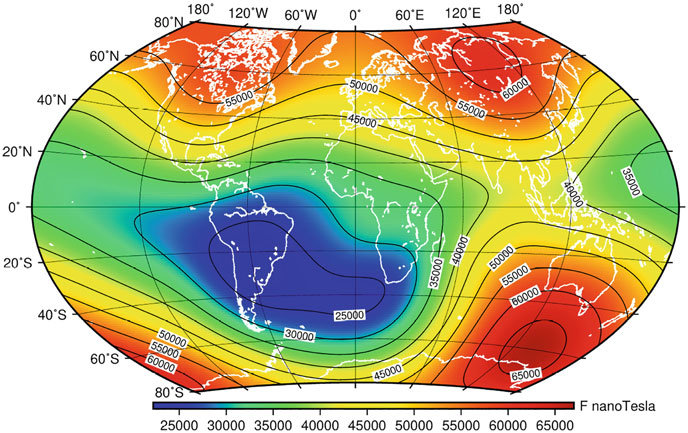
\includegraphics[width = 10cm]{Figures/IGRF-13th.png}
	\caption{The magnitude of geomagnetic field according to the 13th generation of the IGRF model~\cite{koskinen2022radiation}.}
	\label{fig:IGRF13th}
\end{figure*}

\section{Disturbance models}
\label{section: disturbance models}
During orbit, a satellite is exposed to various disturbance torques. It is these torques that cause the modelled attitude to differ from the actual attitude. These torques are therefore modelled and are assumed to influence the attitude of the satellite continuously. Other disturbances that occur only with anomalies are discussed in Chapter~\ref{chap:Anomalies}. Some disturbances are excluded from the simulation environment and only the major sources of disturbance torques are modelled and discussed.

The first disturbance torque is that of the gyroscopic coupling which can be calculated with
\begin{equation}
\mathbf{N}_{gyro} = \boldsymbol{\dot{\omega}}_\mathcal{B}^\mathcal{I} \times (\mathbf{I}\boldsymbol{\dot{\omega}}_\mathcal{B}^\mathcal{I} + \mathbf{h}_w),
\end{equation}
where $h_w$ is the angular momentum of the reaction wheels. The other disturbance torques are discussed in more detail below.

\subsection{Gravity Gradient}
The gravity gradient is caused by both the centrifugal force on the satellite due to the orbit around the Earth as well as the gravitational force. The part of the satellite nearest to the Earth will experience the largest gravitational force and the smallest centrifugal force of the satellite, while the part of the satellite furthest from the Earth will experience the smallest gravitational force and the largest centrifugal force. According to \cite{wertz2012spacecraft} the gravity gradient disturbance torque, $\mathbf{N}_{gg}$ can be calculated as 
\begin{equation}
\boldsymbol{N}_{gg} = 3 \, \omega_\mathcal{O}^2 (\mathbf{z}_{\mathcal{B}} \times \mathbf{Iz}_{\mathcal{B}}).
\end{equation}
The orbit nadir vector is calculated as,
\begin{equation}
\mathbf{z}_{\mathcal{B}} = \boldsymbol{A}^{\mathcal{B}}_{\mathcal{O}} \begin{bmatrix} 0 & 0 & 1 \end{bmatrix}^T.
\end{equation}
Due to the design of the satellite and the positions of the solar panels, the equation for $\mathbf{N}_{gg}$ can not be simplified. The gravity gradient torque is the only torque that can be accurately modelled on-board the satellite, and is therefore also included in the model update of the EKF. $\mathbf{N}_{gg}$ in SBC is shown in Figure~\ref{fig:GravityGradientTorques}.

\textbf{TODO: Change all plots x, y, and z should be in mathbf and the colors should correspond to that of the pitch figure}.

\begin{figure}[!htb]
	\centering
	\def\pgfwidth{10cm}
	\import{Figures/TexFigures/Predictor-None/Isolator-None/Recovery-None/EARTH_SUN-ORC-General CubeSat Model/None/}{Gravity Gradient Torques.pgf}
	
	\caption{Gravity Gradient Torque in SBC}
	\label{fig:GravityGradientTorques}
\end{figure}

\subsection{Aerodynamic Disturbance}
The aerodynamic disturbance torques are cause by air density in the atmosphere creating a force on each individual segment of the satellite~\cite{Steyn2014}. This is significant due to the low Earth orbit (LEO) of the satellite, where the atmospheric density is higher. The aerodynamic disturbance torque, $\mathbf{N}_{aero}$ is therefore a summation of all the torques created by the air force on each segment area, $A_i$. $\mathbf{N}_{aero}$ can therefore be calculated as

\begin{equation}
\begin{aligned}
\mathbf{N}_{aero} = \sum_{i=1}^{n}\Big(& \rho \norm{\mathbf{v}_{\mathcal{B}}}^2 A_i H \{\text{cos}(\alpha_i)\} \, \text{cos}(\alpha_i) \big(\sigma_t (\mathbf{r}_{pi} \times \mathbf{\bar{v}}_{\mathcal{B}}) \\
					 & + \big[ \sigma_nS + (2 - \sigma_n - \sigma_t) \text{cos}(\alpha_i)\big] (\mathbf{r}_pi \times \mathbf{\bar{n}}_i) \big) \vphantom{\norm{\mathbf{v}_{\mathcal{B}}}^2}\Big),
\end{aligned}
\end{equation}
where $n$ is the number of segments of the satellite. The factors that influence the aerodynamic disturbance torque is the atmospheric velocity in SBC, $\mathbf{v}_{\mathcal{B}}$, the atmospheric density, $\rho$, each segment's surface area, $A_i$, and the offset vector between the segment's centre of mass (CoM) and the centre of pressure (CoP), $\mathbf{r}_p$. $H\{x\}$ is the Heaviside function which is equal to $0$ when $x$ is smaller than $0$ and otherwise equal to $1$. $\alpha_i$ is the incidence angle of $\mathbf{v}_{\mathcal{B}}$ on segment $i$, while $\sigma_t$ is the tangential accommodation coefficient and $\sigma_n$ is the normal accommodation coefficient. $S$ is the ratio of molecular exit velocity to $\mathbf{v}_{\mathcal{B}}$ and $\mathbf{\bar{n}}_i$ is the unit inward normal vector of segment $i$ \cite{JansevanVuuren2015}.

The atmospheric density is a function of the distance from the Earth surface. The density model provided by \cite{vallado2001fundamentals} is given as 
\begin{equation}
\rho = \rho_o e^{-\frac{h(t)-h_o}{H}},
\end{equation}
where $\rho_o$ is the reference density at the reference altitude, $h_o$, and $h(t)$ is the satellite's altitude as a function of time and $H$ is the scale height. According to \cite{steyn2011CubeSat} the atmospheric density is $\frac{1}{2}\rho$ during an eclipse. Furthermore $\mathbf{v}_{\mathcal{B}}$ is calculated as
\begin{equation}
\begin{aligned}
\mathbf{v}_{\mathcal{B}} &= \boldsymbol{A}^{\mathcal{B}}_{\mathcal{O}} \boldsymbol{A}_{\mathcal{E}}^{\mathcal{O}} \mathbf{v}_{\mathcal{E}} \\
\text{where}  \qquad \mathbf{v}_{\mathcal{E}} &= \begin{bmatrix} 0 \\ 0 \\ \omega_E \end{bmatrix} \times \mathbf{r}_{sat} - \mathbf{v}_{sat}.
\end{aligned}
\end{equation}

$\sigma_n$ and $\sigma_t$ are both assumed to be equal to 0.8, while $S$ is $\num{0.8}$~\cite{steyn2011CubeSat}. From these equations the aerodynamic disturbance can be calculated and is shown in Figure~\ref{fig:AerodynamicTorques}.
\begin{figure}[!htb]
	\centering
	\def\pgfwidth{10cm}
	\import{Figures/TexFigures/Predictor-None/Isolator-None/Recovery-None/EARTH_SUN-ORC-General CubeSat Model/None/}{Aerodynamic Torques.pgf}
	
	\caption{Aerodynamic Torques in SBC}
	\label{fig:AerodynamicTorques}
\end{figure}

\subsection{Wheel Imbalance}
Since the reaction wheel imbalance is considered to be the most significant disturbance on the reaction wheel, it is the only disturbance torque modelled for this simulation~\cite{bialke1998high}. Although reaction wheels are manufactured with low tolerances, the reaction wheel will have a slight imbalance, since the mass of the reaction wheel will not be perfectly uniform and evenly displaced. 

The static imbalance of the reaction wheel is caused by the reaction wheel CoM offset from the rotational axis. Therefore, to model the static imbalance of the reaction wheels it is assumed that the unevenly distributed mass of the reaction wheel can be simplified to a point mass, $m$, a distance, $r$ from the rotational axis as shown in Figure~\ref{fig:StaticImbalance}. The static imbalance, $U_s$ is equal to $mr$ and this value is provided by the reaction wheel manufacturers.

\begin{figure}[!htb]
	\centering
	\def\svgwidth{10cm}
	\import{Figures/}{StaticImbalance.pdf_tex}
	\caption{Static Imbalance}
	\label{fig:StaticImbalance}
\end{figure}

To determine the resulting torque from the wheel imbalance, the torque generated by each wheel is individually calculated. Consequently, for the reaction wheel in direction $\bar{x}_\mathcal{B}$, $RW_{\bar{x}_\mathcal{B}}$, the force, $F_{s\bar{x}_\mathcal{B}}$, generated by $U_s$ is dependent on the the angular rate, $\omega$, of the reaction wheel as well as the current position of $m$. Therefore, $F_{s\bar{x}_\mathcal{B}}$ can be expressed as

\begin{equation}
\mathbf{F}_{s\bar{x}_\mathcal{B}} = U_s\omega^2 \begin{bmatrix} 0 \\ \text{sin}(\omega t + \phi_s) \\ \text{cos}(\omega t + \phi_s)\end{bmatrix},
\end{equation}

where the current angle of $m$ is defined as $\omega t + \phi_s$, with $\phi_s$ as an arbitrary phase and for the sake of simplification is set to $0$. With $F_{s\bar{x}_\mathcal{B}}$ exerted on $RW_{\bar{x}_\mathcal{B}}$ known, the torque on the satellite can be calculated with the known position vector, $\mathbf{w}_{\bar{x}_\mathcal{B}}$, of $F_{s\bar{x}_\mathcal{B}}$ to the satellite CoM. Therefore, $N_{s\bar{x}_\mathcal{B}}$ can be calculated as

\begin{equation}
\mathbf{N}_{s\bar{x}_\mathcal{B}} = \mathbf{w}_{\bar{x}_\mathcal{B}} \times F_{s\bar{x}_\mathcal{B}}.
\end{equation}

This is calculated for each reaction wheel to determine the resulting static imbalance disturbance torque on the satellite. Another aspect of the reaction wheel imbalance is also modelled, namely the dynamic imbalance. The dynamic imbalance is caused by the principal inertia of the reaction wheel being misaligned with the rotational axis. This can be simplified to two equal point masses, $m$, with an axial displacement, $d$, and distance, $r$, from the rotational axis. These two masses are $\num{180}^o$ apart with respect to the rotational axis and, consequently, create two forces equal in magnitude and in opposite directions. The dynamic imbalance is graphically represented in Figure~\ref{fig:DynamicImbalance}.

\begin{figure}[!htb]
	\centering
	\def\svgwidth{10cm}
	\import{Figures/}{DynamicImbalance.pdf_tex}
	\caption{Dynamic Imbalance}
	\label{fig:DynamicImbalance}
\end{figure}

The dynamic wheel imbalance torque, $\mathbf{N}_{d\bar{x}_\mathcal{B}}$, for $RW_{\bar{x}_\mathcal{B}}$ can be calculated as 
\begin{equation}
\mathbf{N}_{d\bar{x}_\mathcal{B}} = U_d\omega^2 \begin{bmatrix} 0 \\ \text{sin}(\omega t + \phi_d) \\ \text{cos}(\omega t + \phi_d)\end{bmatrix}.
\end{equation}
where $U_d = mrd$ as the dynamic imbalance. Both $U_d$ and $U_s$ are provided by the manufacturer and based on the reaction wheel as discussed in Section~\ref{section:Actuators}. The net wheel imbalance torque from both the static and dynamic wheel imbalance is provided in Figure~\ref{fig:Wheel disturbance Torques}.

\begin{figure}[!htb]
	\centering
	\def\pgfwidth{10cm}
	\import{Figures/TexFigures/Predictor-None/Isolator-None/Recovery-None/EARTH_SUN-ORC-General CubeSat Model/None/}{Wheel disturbance Torques.pgf}
	
	\caption{Wheel disturbance torques in SBC}
	\label{fig:Wheel disturbance Torques}
\end{figure}


%\section{Constellations}
%Explain the design of the satellite constellations and the algorithms to run communicate between satellites.
%
%\begin{algorithm}
%	
%	\SetKwInOut{Input}{Input}
%	\SetKwInOut{Output}{Output}
%	
%	\SetKwData{Left}{left}
%	\SetKwData{This}{this}
%	\SetKwData{Up}{up}
%	\SetKwFunction{Union}{Union}
%	\SetKwFunction{FindCompress}{FindCompress}
%	
%	\Indm
%	\Input{Description of the input to the algorithm.}
%	\Output{Description of the output from the algorithm.}
%	\Indp
%	
%	\BlankLine
%	
%	\emph{Initialize hyperparameters}\;
%	Get initial data from satellite\\
%	Update positions of each satellite\\
%	\For{$i\leftarrow 1$ \KwTo $N$}{
%		Determine $k$-nearest satellites to $satellite_i$ from the positions\\
%		Select data from nearest satellites\\
%		Send nearest satellites predictions and data to $satellite_i$\\
%		Retrieve data from $satellite_i$ and fault predictions of $k$-nearest satellites\\
%	}
%	Update position of $satellite_i$\\
%	Update data of $satellite_i$
%	
%	\caption[Do not end short caption with full-stop]{Algorithm example}
%	\label{alg}
%	
%\end{algorithm}


%\section{Typical Faults}
%For the simulation of the satellite and the induced faults to train and test various anomaly detection methodologies a database of typical faults is required. \cite{tafazoli2009study} made a study of the percentage of failure per subsystem. 
%
%\subsection{Probability of Fault Occurence}
%The occurrence of a fault depends on the reliability of that equipment. \cite{Guo2014} studied the reliability of small satellites and calculated the parameters for the Weibull distribution based on real data. To model the probability of a fault to occur the probability density function is used \cite{Jones2017}.
%
%This probability however is small and for the training of the system the data is too sparse for the computational abilities of any regular PC. Thus the probability of a failure during training is fixed to $1/1000000$ to produce the data required for the anomaly detection with a million test samples.
%
%\subsection{Set of faults}
%A set of typical faults for the ADCS is shown in Table~\ref{ADCS fault table}. 
%
%\newpage
%\begin{sidewaystable}[]
%	\label{ADCS fault table}
%	\begin{tabular}{|l|c|l|l|l|l|}
%		\hline
%		\multicolumn{6}{|c|}{\textbf{Internal Faults}} \\ \hline
%		\textbf{Fault classes} &
%		\multicolumn{1}{l|}{\textbf{\begin{tabular}[c]{@{}l@{}}Failure rate \\ per hour\end{tabular}}} &
%		\textbf{Fault causes} &
%		\textbf{References} &
%		\textbf{Possible effect} &
%		\textbf{Possible permutations} \\ \hline
%		\multirow{4}{*}{Reaction wheels} &
%		\multicolumn{1}{l|}{\multirow{4}{*}{2.5E-7 \cite{Spilhaus1987}}} &
%		\begin{tabular}[c]{@{}l@{}}Reaction wheel electronics \\ fail\end{tabular} &
%		\cite{allen2012satellite} \cite{Jacklin2019} &
%		\begin{tabular}[c]{@{}l@{}}Does not respond \\ to control inputs\end{tabular} &
%		\begin{tabular}[c]{@{}l@{}}Momentum remains the same \\ or decreases slightly due to \\ friction\end{tabular} \\ \cline{3-6} 
%		&
%		\multicolumn{1}{l|}{} &
%		Overheated reaction wheel &
%		\cite{Wintoft} &
%		Decrease in speed &
%		1\% of initial speed per second \\ \cline{3-6} 
%		&
%		\multicolumn{1}{l|}{} &
%		\begin{tabular}[c]{@{}l@{}}Catastrophic failure (cause \\ unknown)\end{tabular} &
%		\cite{Choi2011} &
%		Stops rotating &
%		0 \\ \cline{3-6} 
%		&
%		\multicolumn{1}{l|}{} &
%		\begin{tabular}[c]{@{}l@{}}Increase in rotation speed \\ (Unknown cause)\end{tabular} &
%		\begin{tabular}[c]{@{}l@{}}Gerhard Janse \\ van Vuuren\end{tabular} &
%		\begin{tabular}[c]{@{}l@{}}Wheel speed \\ increases\end{tabular} &
%		\begin{tabular}[c]{@{}l@{}}Between 90-100\% of maximum \\ wheel speed\end{tabular} \\ \hline
%		Magnetorquers &
%		\multicolumn{1}{l|}{ADCS fault table8.15E-9 \cite{Spilhaus1987}} &
%		Polarities are inverted &
%		\cite{Crowell2011} &
%		Incorrect rotation &
%		\\ \hline
%		\multirow{2}{*}{Magnetometers} &
%		\multicolumn{1}{l|}{\multirow{2}{*}{8.15E-9 \cite{Spilhaus1987}}} &
%		Unknown &
%		\begin{tabular}[c]{@{}l@{}}Gerhard Janse \\ van Vuuren\end{tabular} &
%		Stops reacting &
%		\begin{tabular}[c]{@{}l@{}}Provides no feedback or the \\ output remains constant\end{tabular} \\ \cline{3-6} 
%		&
%		\multicolumn{1}{l|}{} &
%		\begin{tabular}[c]{@{}l@{}}Magnetometers and magne-\\ torquers interfered with \\ each other\end{tabular} &
%		\cite{Jacklin2019} &
%		\begin{tabular}[c]{@{}l@{}}Noise on magneto-\\ meters and noise \\ on control of mag-\\ netorquers\end{tabular} &
%		\begin{tabular}[c]{@{}l@{}}Between x3 and x5 times the \\ normal noise magnitude \\ Guassian distribution\end{tabular} \\ \hline
%		Earth Sensor &
%		- &
%		Unknown &
%		\cite{Robertson2019} &
%		\begin{tabular}[c]{@{}l@{}}Noisy Earth Sensor \\ effected pointing \\ accuracy\end{tabular} &
%		\begin{tabular}[c]{@{}l@{}}Between x5 and x10 times the \\ normal sensor noise based on \\ Guassian distribution\end{tabular} \\ \hline
%		\multirow{2}{*}{Sun sensor} &
%		\multirow{2}{*}{-} &
%		\begin{tabular}[c]{@{}l@{}}Cross-wired during instal-\\ lation\end{tabular} &
%		\cite{Crowell2011} &
%		\begin{tabular}[c]{@{}l@{}}Erroneous \\ measurements\end{tabular} &
%		Uniform random values \\ \cline{3-6} 
%		&
%		&
%		Unknown &
%		\cite{Jacklin2019} &
%		Sun sensor fails &
%		output is 0 \\ \hline
%		Star tracker &
%		- &
%		\begin{tabular}[c]{@{}l@{}}Shutter on star tracker is \\ closed\end{tabular} &
%		\cite{Crowell2011} &
%		Star tracker fails &
%		output is 0 \\ \hline
%		Overall control &
%		- &
%		\begin{tabular}[c]{@{}l@{}}Incorrect control law or \\ variation \\ thereof\end{tabular} &
%		\begin{tabular}[c]{@{}l@{}}Gerhard Janse \\ van Vuuren\end{tabular} &
%		\begin{tabular}[c]{@{}l@{}}Angular velocity \\ suddenly increases \\ or decreases or \\ oscillation results\end{tabular} &
%		\begin{tabular}[c]{@{}l@{}}Increase to 75 - 100\% \\ Decrease to 0 - 25\%\\ Oscillates\end{tabular} \\ \hline
%		\multirow{3}{*}{\begin{tabular}[c]{@{}l@{}}Common data \\ transmission errors\end{tabular}} &
%		\multirow{3}{*}{-} &
%		Sign flip &
%		\cite{Crowell2011} &
%		Processor-based &
%		\begin{tabular}[c]{@{}l@{}}Processor outputs and/or \\ inputs experience a sign flip\end{tabular} \\ \cline{3-6} 
%		&
%		&
%		Bit flip &
%		N/A &
%		&
%		\begin{tabular}[c]{@{}l@{}}Processor outputs and/or \\ inputs experience a bit flip flip\end{tabular} \\ \cline{3-6} 
%		&
%		&
%		Insertion of zeros &
%		\cite{Jacklin2019} &
%		&
%		\begin{tabular}[c]{@{}l@{}}Processor outputs and/or inputs \\ experience an insertion of a zero\end{tabular} \\ \hline
%		\begin{tabular}[c]{@{}l@{}}Possible sensors \\ errors\end{tabular} &
%		- &
%		Unknown &
%		N/A &
%		High sensor noise &
%		\begin{tabular}[c]{@{}l@{}}Between x5 and x10 times the \\ normal sensor noise based on \\ Guassian distribution\end{tabular} \\ \hline
%	\end{tabular}
%\end{sidewaystable}
%
%\newpage